So far I have demonstrated that it is possible to design a type system for most
of real-world C. In particular, such a type system supports resource management
in the presence of complex control flow, variable scoping and aliasing, and has
a conceptually simple extension to handle loose evaluation order.

One of the features I glossed over was the subtle and complex rules regarding
pointer manipulations, which cannot be ignored or simplified away in practice,
especially given \kl{CN}'s headline goal (\cref{sec:cn-intro}) to work
correctly above pre-existing C programs and observed behaviour.

The subtlety around observed behaviour for pointer manipulations stems from the
competing forces which shaped C.\sidenote{Inherited portability requirements,
proximity to hardware, and the desire for more aggressive optimisations.} As I
explained in \cref{sec:c-lang}, a completely concrete view of pointers would
invalidate fundamental optimisations we would like to perform on our code, but
a completely abstract view where pointers cannot alias each other is simply
incompatible with C's ability to take addresses of variables and compute with
pointers (incremet, calculate offsets, cast them to and from integers).

Whilst many aspects of C are specified using an elaboration, the representation
of pointers, and the choice of rules for manipulating them, are factored out
into a \emph{memory interface}. This interface is visible in
\cref{fig:effectful-core-grammar}: the memory operations $\mathit{memop}$ and
the memory $\mathit{actions}$; a \intro{memory object model}\sidenote{Named so
to distinguish it from a memory model in a concurrency setting.} is an
implementation of that interface.

Remember that C has a lot of different stakeholders, and so a memory model
which is acceptable to the standards committee needs to walk a fine line
between being concrete enough to enable as many low-level idioms as possible,
whilst being abstract enough to permit as many optimisations as possible. The
key concept which enables this is the idea of pointer \intro{provenance},
tracking where a pointer came from. With this, because C allows casting to and
from integers, the question naturally arises about whether this provenance
should be tracked via integers or not. Unfortunately, that is not the only
choice point involved in coming up with an acceptable memory object model;
\sidetextcite{memarian2022cerberus} documents and explains the trade-offs
between this and other choices.

Any set of choices must nagivate the tension between allowing
low-level idioms relied upon by existing code, allowing opportunities for
optimisations exhibited by existing compilers, and limiting the scope of both.
The cost of doing so (in a consistent manner\sidenote{None of the memory models
discussed are consistent with all observed behaviour, and it is not clear that
there is a consistent one which would be.}) is that the so far preferred (but
not yet officially adopted) memory object model,
\kl{PNVI-ae-udi},\sidenote{Provenance not tracked via integers, for addresses
which are exposed and provenances user-disambiguated. I will explain this imminently.} is a
complex minefield of \kl{UB} no human should be expected to navigate
unassisted.

\kl{PVNI-ae-udi} is complex enough that even implementing it in a C
verification tool is undesirable, especially because in that context, it is
reasonable to place a small extra burden of annotation on the user if it
simplifies verifying the code. This is the motivation behind the development of
\kl{VIP},\sidecite{lepigre2022vip} a memory model which is sound with respect
to PNVI-ae-udi,\sidenote{Quoting from the paper, ``every PNVI-ae-udi step can
be simulated by a VIP step, and that every step that raises
\kl[UB]{undefined behaviour} in PNVI-ae-udi also raises \kl[UB]{undefined
behaviour} in VIP.''} but simpler (it is fine to reject more programs, i.e.\
have more \kl{UB}).

\kl{VIP} as a memory model is \emph{simpler}, but it is not trivial. It is
defined operationally as a step relation between concrete (i.e.\ not symbolic)
heavily structured heaps, and the steps have complex premises.

In this part, I will detail the challenges and choices I faced in designing,
formalising and implementing \kl{CN-VIP}, the memory model of \kl{CN} as a scheme
within the formalised and implemented type systems.
\begin{itemize}
    \item \textbf{Expressiveness vs simplicity.} \kl{VIP} makes a particular
        choices about its representation of pointers and integers, and relatedly
        about the idioms it supports. I will explain it, and the other
        design around it, both simpler and more expressive. In particular,
        I will explain important and subtle complexities around round-trip casts,
        \cinline{memcpy} and \cinline{memcmp}, which are handled in
        \kl{VIP}/\kl{PNVI-*} test-suite, but not discussed.
    \item \textbf{Integration into \kl{Kernel CN}.} As I mentioned in
        \cref{sec:res-terms}, the novel structure for heaps abstracts away
        some aspects of its representation. I will explain how I adapted the
        static and dynamic semantics to use \kl{VIP}, and proved the new system
        sound with less repeated effort than typical.
    \item \textbf{Implementation in \kl{CN}.} I will explain how I incrementally
        developed, gated and deployed a complex change to memory model of \kl{CN}.
        By the time I had designed and formalised \kl{CN-VIP}, \kl{CN} had
        users, a tutorial, a test-suite and a continuous integration pipeline,
        so I had to be careful in adding support for \kl{VIP}, avoid difficult
        code merges and test updates.
    \item \textbf{Impact on annotations and performance.} Finally, I will explain
        how switching over to \kl{CN-VIP} (without round-trip casts) impacted
        the annotations and performance on existing \kl{CN} tests and tutorial
        examples.
\end{itemize}

\chapter{Memory Object Models, explained}\label{chap:mem-model-explained}

From the perspective of \kl{Core} and \kl{ResCore}, the memory object model
(\cref{fig:mem-model-intf}) is simply a choice of representation of pointers,
and the interface specified in the memory operations $memop$, and memory
$\mathit{actions}$.\sidenote{Plus some extra primitives to detect races between
unsequenced expressions, which I will ignore.}

\begin{marginfigure}
    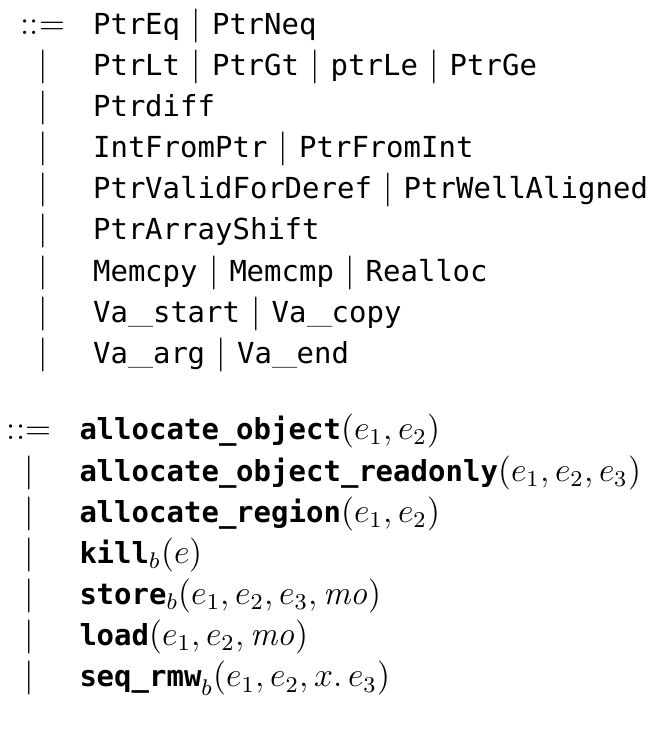
\includegraphics{figures/mem-model-intf}
    \caption{Memory model interface of \kl{Core}.}\label{fig:mem-model-intf}
\end{marginfigure}

The key concept which begins this brief overview of memory object models is
that of provenance. To optimise our code, compilers would like to assume that
not all pointers that a programmer can magically create (a) are valid, i.e.\
point to a live allocation (b) can alias any other live allocation in scope.

Let us revisit the example from \cref{fig:ptr-from-int}, reproduced in
\cref{fig:mem-model-ptr-from-int} for convenience. It shows a simple function
which takes an integer as an argument, assigns the number 5 to a local, and the
prints the value of that local, with some intervening pointer shenanigans.
Despite the fact that there is no data flowing between \cinline{k} and
\cinline{i}, the mere fact that the address of \cinline{j} was taken (and
``exposed'' via its assignment to an integer \cinline{k}) is enough to make the
compiler wary that the pointer \cinline{p} could alias \cinline{j} and thus
disable constant propagation.

\begin{marginfigure}
    \centering
    \cfile{code/pointer_from_integer_1ie.c}
    \caption{Example pointer\_from\_integer\_1ie.c.}\label{fig:mem-model-ptr-from-int}
\end{marginfigure}

Explain pointers in excruciating detail, and why we need provenance for
optimisations.

Why do we care about provenance, why are pointers not just addresses

Common sub-expression elimination, copy-propagation, etc.

\section{Explaining PNVI-ae-udi and VIP}

Why you need provenance.

\section{Design Space}

Alternatives

\begin{figure}[h]
    \centering
    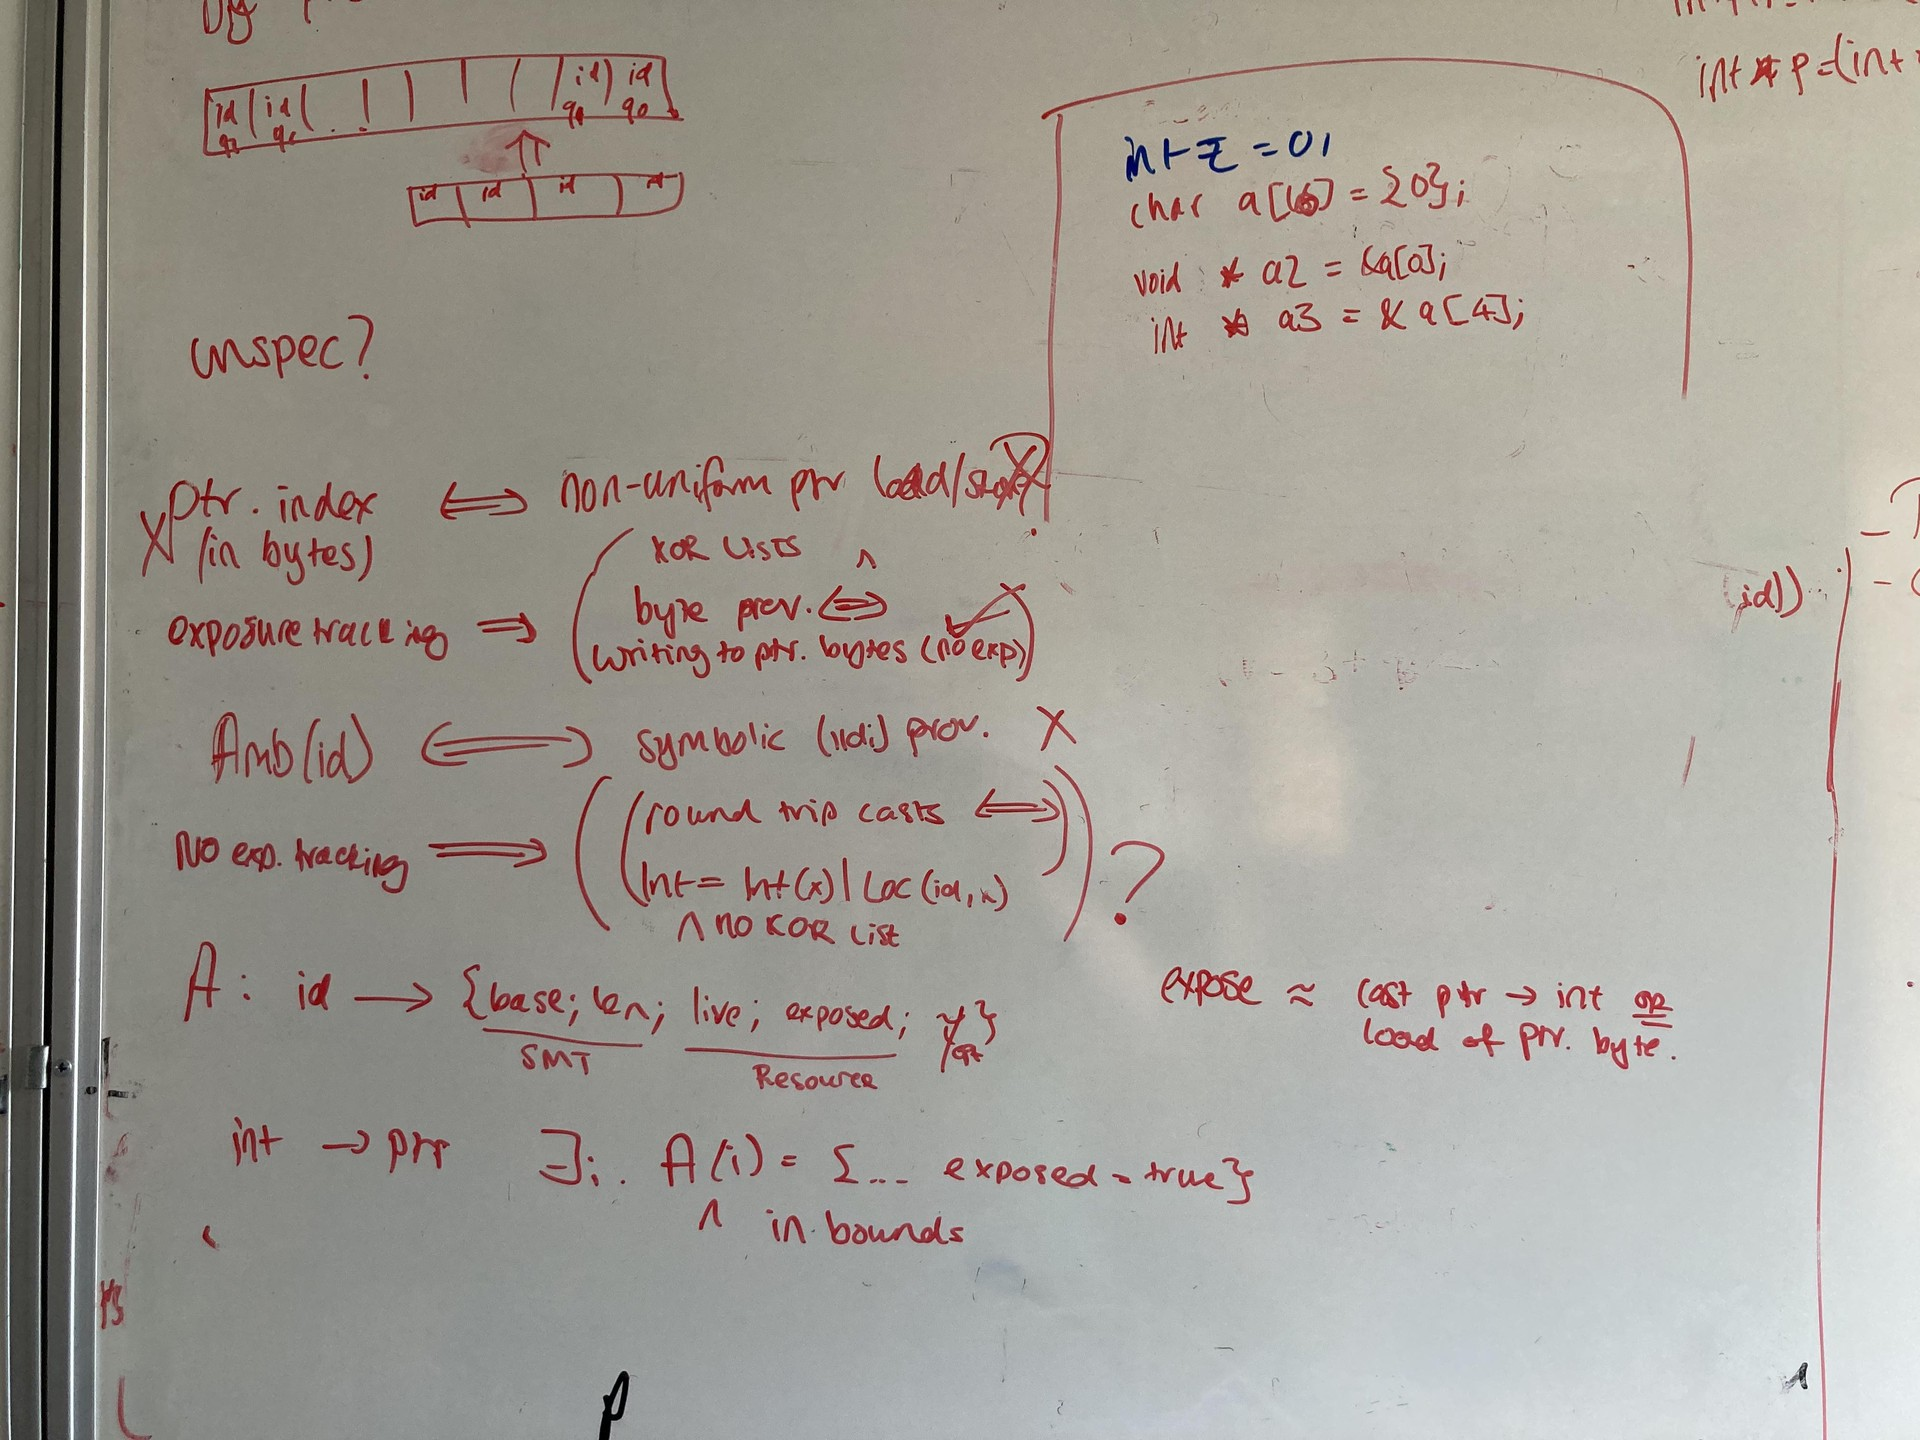
\includegraphics[width=\textwidth]{../misc/type-system-options.jpg}
\end{figure}

\section{CN-VIP}\label{sec:cn-vip}

\section{Soundness}\label{sec:cn-vip-soundness}

\section{Implementation}

Performance graph

\begin{figure}[h]
    \centering
    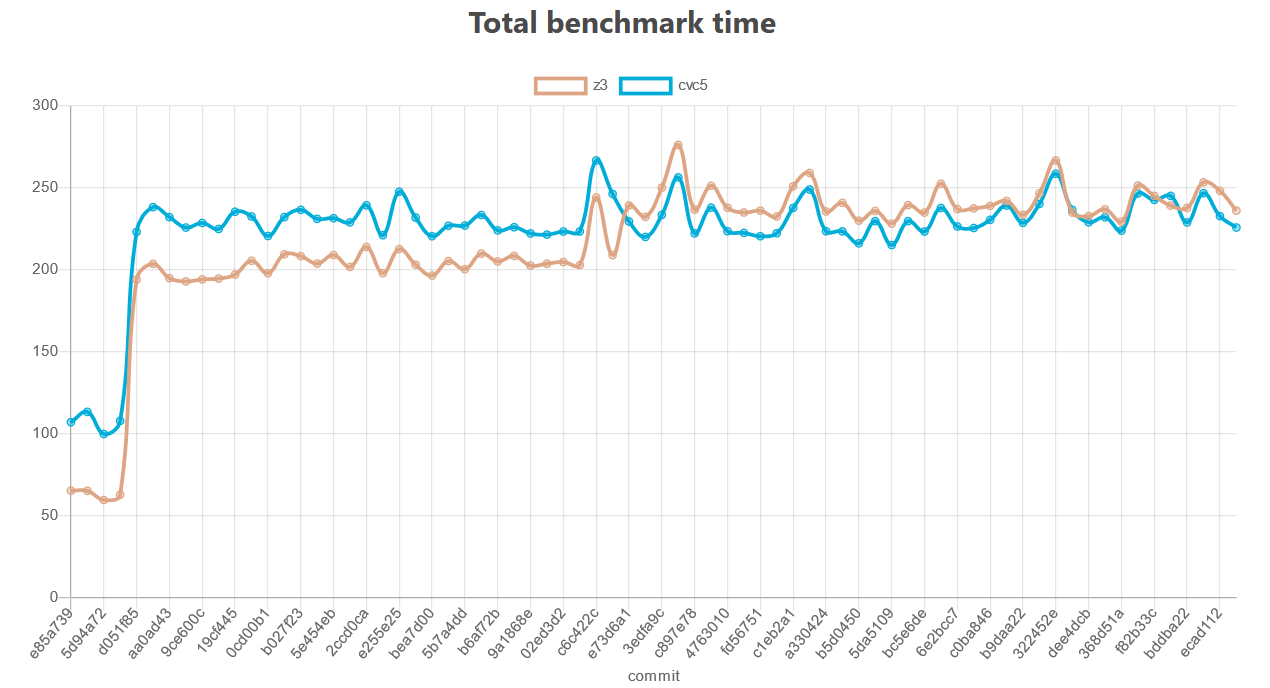
\includegraphics[width=\textwidth]{../misc/vip-performance-hit.png}
\end{figure}

\url{https://rems-project.githb.io/cerberus/dev/bench/}

\section{Translating resource lemmas}\label{sec:trans-res-lemmas}

Is there a reason, in the discussion about Cassia's PhD, we thought all of
Cerberus needed to be shoved into Iris instead of just a trace of memory model
(and eventually, concurrency) events?

irisification (cf
\url{https://people.mpi-sws.org/~dreyer/papers/iris-ground-up/paper.pdf}).  Either
just the resource algebra or (as DM suggests) also the abstract language of
memory model interface events: which one let one formalise the primitive
resource-context manipulations that CN does (conceivably extractably).

I think a sufficient halfway point would be the language of traces memory
events i.e.\ memory model as the dynamics. Resource algebra would be CN's view
of resources. Resource lemmas are then just statements saying that one resource
represents exactly the same heap as another resource (skips). Changes to the
resource algebra because of memory events (which we could introduce unsoundness
in CN) would be proved sound in Iris.

As a bonus, we could even formalise and prove sounds the inference procedures
CN uses (and with some engineering to handle SMT, even extract from Rocq).

The inference I'm talking about is resource context manipulations: checking if
we can pack or unpack predicates, if an owned is in the context, shifting
indices in and out of iterated predicates, exploding and imploding structs.
These operations don't require core structure.

Even if full extraction of the inference algo is not feasible (it would
involves standard data structures + SMT FFI), having a defined set of resource
manipulation primitives proved sound and extracting those (just standard data
structure manipulations), or even just proving the primitives sound and using a
similar interface would increase confidence.

If ones reads the above in reverse, it even provides a gradual migration path
which doesn't commit us to any next step and allows us to see how far
extraction can take us.

If the inference algs or the primitives are formalised, then we can iterate on
cleverer  inference schemes with a strong safety net

I think it will become more valuable as soon as we start having fancier things
like higher-order resources, locks, fractional permissions. At that point,
checking the steps/moves that any inference algorithm could take would get
closer to essential.

Even if an arbitrary inference algorithm is not stable, the steps available and
the shape of the resources should be more so, and that is worth at least
creating a clean abstraction for (and then pen-paper soundness, and then
mechanised soundness).

Noted and agreed that anything mechanised takes longer than one wants/expects
and that extraction is a pain. But this gives us a concrete use-case,
reasonable sequence of experiments and a clear idea of the benefits and costs.

